% !TeX spellcheck = en_US
\documentclass[10pt,letterpaper]{article}
\usepackage[latin1]{inputenc}
\usepackage{amsmath}
\usepackage{amsfonts}
\usepackage{amssymb}
\usepackage{graphicx}
\usepackage{url}
\author{Andrew Rosen}
\title{Group Project Report: siRNA Generator}
\date{}
\begin{document}

\maketitle

\section{Overview}
I will first discuss the motivation for our work and our group's broad objective.


\subsection{Motivation}
Our primary motivation for our project was the 2014 Ebola outbreak.
There are five identified species of the Ebolavirus, four of which directly affect humans: Bundibugyo, Ta\"{\i}, Sudan, and Zaire \cite{centers20152014}.
The last, the Reston virus, does not harm humans.
The Zaire ebolavirus is the most deadly and the one responsible for the current outbreak, the most deadly to date.

%symptionm
Symptoms of Ebola virus disease (EVD) include: fever, chills, fatigue, weakness, muscle/join pain,  vomiting, reddened eyes, and hemorrhaging \cite{team2014ebola} \cite{wongcharacterization}.
These symptoms appear within eight to ten days, on average \cite{centers20152014}.

This most recent outbreak primarily affected people in Guinea, Liberia, and Sierra Leone, with additional cases reported in Nigeria, Mali, and Senegal (Figure \ref{fig:west-africa-distribution-map}) \cite{centers20152014}.
Thus far, there have been an estimated 25,907 infected in 2014 outbreak, and nearly 11,000 people have succumbed to the disease \cite{centers20152014}.
Two cases of Ebola were imported to the United States and was spread to two nurses. 
This, plus cases Spain and the United Kingdom sparked a large level of concern worldwide  \cite{levin2015ebola} \cite{ready}.

\begin{figure}
\centering
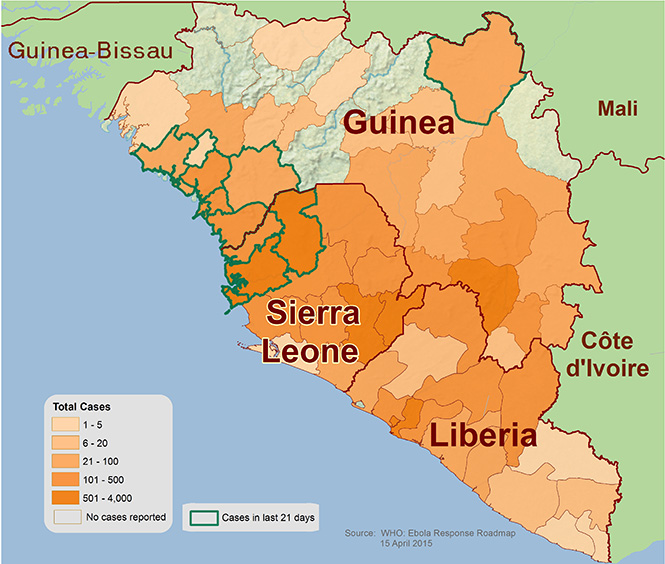
\includegraphics[width=0.5\linewidth]{west-africa-distribution-map}
\caption{Map of total cases of the 2014 Zaire Ebolavirus outbreak. Source: Center for Disease Control \cite{centers20152014}.}
\label{fig:west-africa-distribution-map}
\end{figure}


% prevention
Ebola can be fought, and the most effective method is prevention.
Ebola does not spread easily when compared to other viruses such as influenza.
Infection requires contact with the bodily fluids of a infected person who is displaying symptoms of Ebolavirus disease \cite{wongcharacterization} \cite{team2014ebola}.
Thus, the most effective way currently available is to quarantine the infected individuals and find those who have had contact with the infected \cite{team2014ebola}.
Meanwhile, research into various treatments such as vaccines \cite{geisbert2015emergency} or siRNAs \cite{lipid} has had immense interest due to the severity of this outbreak.


\subsection{Our approach}
We chose to create a tool to design siRNA to fight viruses since a couple of group members were involved in active research on siRNA and were very familiar with it.
siRNA is short for small interfering RNA or silencing RNA as it interferes with or silences the expression of a specific sequence it matches up with.
This specificity makes siRNA highly applicable to cancer treatment \cite{chen2010noparticles}, gene therapy \cite{kim2006peg}, and viral treatment \cite{gitlin2002short}.


Our idea has merit, given that research is being actively done on siRNA Ebola treatments \cite{lipid} \cite{kugelman2015evaluation} \cite{geisbert2010postexposure}.
In a study published in 2010 in the Lancet, Geisbert \textit{et al} \cite{geisbert2010postexposure} successfully tested a post-exposure siRNA treatment which helped protect against Zaire Ebolavirus in primates.

%Generalize it.
Needless to say, a tool for evaluating a single genus of viruses to create a siRNA to combat it, such as ebolaviruses, is highly useful, but is rather limited in scope.
As a result, we chose to create a system which could analyze any group of viruses for a conserved region and designed siRNA to interfere with it.

\section{Contributions}

In this section, I will talk about the division of work between each member of the group and how I implemented my portion of the work.


\subsection{Assigned Tasks}
Our group separated into three rough groups to tackle each of the three tasks we identified.

The first group was tasked with creating a script to identify the conserved region within the species of viruses.
These conserved regions would then be compared against the human genome using BLAST \cite{blast}.
Any sequence that was shared with the human genome would be filtered out of output for the next group, since by targeting that sequence with an siRNA, it could potentially target that sequence in humans.\footnote{This is generally considered a bad idea as I understand it.}
These sequences are output as a FASTA file.

The second group takes the conserved regions that did not show up in the human genome and uses those to design siRNA to bind with the virus's mRNA.
The resulting siRNA needs to then be compared against the human genome, for the same reasons the first group performed a check.
This would output a FASTA file containing the siRNA sequences that would target the genus of virus.
These potential siRNA should be further analyzed for any consequences.
A member of the group also implemented an algorithm to estimate the amount of mutations it would take for the virus to render the siRNA treatment ineffective.


I was the third group and my responsibilities were quite broad.
\begin{itemize}
	\item I needed to write a web application to accept a FASTA file from the user.
	This file would then be passed the beginning of the first group's code. 
	I could accomplish this by spinning up a thread that called the first function needed to run.
	\item I needed to ensure that the publicly accessible web application did not have write capabilities on the server other than writing the file.\footnote{And I just thought of an attack!  I could upload a very, very, large file.  I'm not sure what this would do, but it would probably not be good.} 
	\item I was to help setup the webserver we would use for our application: \texttt{apollo}.\footnote{A highly germane name for the server, since Apollo's portfolio includes plagues and medicine.}
	\item I needed to ensure the rest of the group had the tools they needed to run their python programs.
	\item I made myself available to each of our group members to aid with debugging.
\end{itemize}
In summary, I needed to do some web programming and act as administrator for our server.



\subsection{Implementation}
I worked with Brendan to install Ubuntu 14.04 LTS on the server. 
This was a fairly trivial task.

I then had to acquire the various pieces of software we needed, which included:

\begin{itemize}
	\item BLAST \cite{blast} and clustalw \cite{thompson2002multiple} for sequence alignment.
	\item Biopython \cite{cock2009biopython}, which contains many useful biology related python scripts and classes.
	\item RNAfold \cite{lorenz2011viennarna},  which predicts the secondary structures of RNA
	\item I also obtained the necessary human genome files to perform sequence alignment from NCBI.
\end{itemize}

I will talk specifically about the goal of each part of the application and my implementation of it.
You can find my code on github: 

\url{https://github.com/abrosen/bioinf/tree/master/website/}

\subsubsection{Application}
The first part of the application is the part the user sees.
I created a fairly simple webserver using Python, which I named \texttt{listener}.
The \texttt{listener} listens on port 8000 for an incoming get request and then serves a webpage (Figure \ref{fig:website}). 
The webpage is stored as a string in \texttt{listener}.

%insert screenshot here
\begin{figure}
\centering

\includegraphics[width=0.5\linewidth]{website}
\caption{The upload form. This is output from the \texttt{listener}.  
	The user uploads a FASTA file and their email address.
	This information is stored in the server on files and read by \texttt{scheduler}.
	}
\label{fig:website}
\end{figure}



Once \texttt{listener} gets a POST from the user, the \texttt{listener} timestamps the received file and email.
They are stored locally and the FASTA file will be read by the \texttt{scheduler}.
This separation of exists to prevent malicious users from having write access by compromising the python program that will be performing all the computations.


\subsubsection{Scheduler}
The scheduler scans the current directory for new files.
Upon finding new FASTA files, it feeds them to the first part of the siRNA sequencer.

In order to do this in a responsive manner, I have \texttt{scheduler} check every 10 seconds for a new file and boot up a new thread.
The thread is not a daemon and it will run independently of \texttt{scheduler} in the event \texttt{scheduler} crashes.

Once the scripts are done executing, the \texttt{scheduler} emails the user with the results.
The emails are sent from the server to the Computer Science department's server, which forwards the mail to where it needs to go.



\section{Evaluation}

\subsection{Test Case}
We planned on using a FASTA file of the five species of the Ebolavirus as our initial input and test case for the entire program.
For my part of the program, I tested \texttt{listener} by uploading various files to \texttt{apollo} via the webpage form and verifying they were intact on the server side.
The most tedious part I had to test was the email portion. 
Most mail servers I tried to use did not accept connections from computer.
I was only able to send mail directly to the department's server when I was logged in to the campus VPN.

\subsection{Deliverables}
A deadline for combining the code was set for April 19th and not met.
There are a number of reasons for this, but I do not believe that the problem was too difficult or large.

I believe the main problem was that our group fractured into many groups of one member, which resulted lack of communication.
Each member made their own assumptions about how the components their program were connecting to would work, even though we had determined that FASTA was the common input and output between files.
I had assumed that we would be using classes from biopython to store the data intermediately, but I must have not expressed this properly to the members of the group and should have made more of an effort to do so.

We did meet later and managed to consolidate our code.  
The individual pieces work, although they don't work \textit{together}.
The final code can be seen on my GitHub repo, where we have my webserver code, \texttt{group\_one\_code.py}, and \texttt{siRNA.py}.

\bibliography{report}
\bibliographystyle{plain}

\end{document}